\documentclass{beamer}

\usepackage{graphicx} % Required for inserting images

\usepackage{beamerthemesplit}

\usepackage{xmpmulti}
\usepackage{animate}
\usepackage{amsmath}
\usepackage{physics}
\usepackage{xcolor}
\usepackage{graphicx}
\usepackage{fontawesome}

% \usepackage{svg}
\usepackage[inkscapeformat=png]{svg}


\usetheme{Copenhagen}
\useoutertheme{infolines}

\title[Systematic Description of W.M.]{A Systematic Description of the Wobbling Motion in Odd-Mass Nuclei Within a Semi-Classical Formalism}


% old author setup
% \author[Robert Poenaru]{%
%     \parbox[t]{0.5\textwidth}{%
%         \textbf{Author} \\
%         Robert Poenaru\inst{1} \inst{2}
%     }%
%     \parbox[t]{0.5\textwidth}{%
%         \textbf{Scientific Coordinator} \\
%         Prof. Em. Dr. A. A. Raduta\inst{2}
%     }%
% }
% \institute[DFT]{
% \inst{1} Doctoral School of Physics, UB \and %
% \inst{2} Department of Theoretical Physics, IFIN-HH
% }

% manual override for a side-by-side author view
\author[Robert Poenaru]{%
    \parbox[t]{0.45\textwidth}{%
		\centering
		\textbf{PhD Candidate} \\
		Robert Poenaru\texorpdfstring{$^{1,2}$}{(1,2)}
    }%
    \parbox[t]{0.45\textwidth}{%
		\centering
        \textbf{Scientific Supervisor} \\
        Prof. Dr. Em. A. A. Raduta\texorpdfstring{$^{2}$}{(2)}
    }%
}
\institute[IFIN-HH]{\texorpdfstring{$^{1}$}{1}Doctoral School of Physics, UB \\ \texorpdfstring{$^{2}$}{2}Department of Theoretical Physics, IFIN-HH}

\date[\today]{\textit{A presentation for the degree of Doctor of Philosophy}\vspace{0.2cm} \\ \today} % Presentation date or conference/meeting name, the optional parameter can contain a shortened version to appear on the bottom of every slide, while the required parameter value is output to the title slide



%%%%%%%%%%%%%%%%%%%%%%%%%%%%%%%%%%%%%
%%%%%%% start of the document %%%%%%%
%%%%%%%%%%%%%%%%%%%%%%%%%%%%%%%%%%%%%

\begin{document}

% trick to show a the first slide without the header
{\setbeamertemplate{headline}{}
\begin{frame}
	\titlepage % Output the title slide, automatically created using the text entered in the PRESENTATION INFORMATION block above
\end{frame}}

\begin{frame}
    \frametitle{TOC}
    \tableofcontents
\end{frame}

\section{Aim and Motivation}

\begin{frame}
    \frametitle{Aim}
    \begin{block}{\faClipboard\ Research Objectives}
        \begin{itemize}
            \item Extend the current interpretation of the \textbf{nuclear triaxiality} in the context of its unique fingerprint: \textbf{Wobbling Motion} % {\footnotesize\emph{from a theoretical standpoint}}
            \item Adopt a framework that is as close as possible to \textbf{classical physics}.
            \item Provide new formalisms for the phenomena related to \textbf{nuclear deformation}.
        \end{itemize}
    \end{block}
    \begin{exampleblock}{\faClipboard\ Objectives exclusive to the thesis}
        \begin{itemize}
            \item Give the reader enough context towards a better understanding of the underlying concepts, methods, and results.
            \item \faGithub\ create a completely \emph{open-source} project.
        \end{itemize}
    \end{exampleblock}
\end{frame}

\begin{frame}
	\frametitle{Motivation}
    \vspace{-0.3cm}
    \begin{itemize}
        \item \textbf{Nuclear Triaxiality} has become a \emph{hot topic} within the scientific community.
        \item Identifying nuclei with triaxial deformations represents a real \textbf{experimental} and \textbf{theoretical} challenge.
        % \item Experimental side: large setups, complex electronics, 
        % \item Theoretical side: cumbersome models, approximations, abstractions...
    \end{itemize}
    \vspace{-0.2cm}
    \begin{figure}
        \centering
        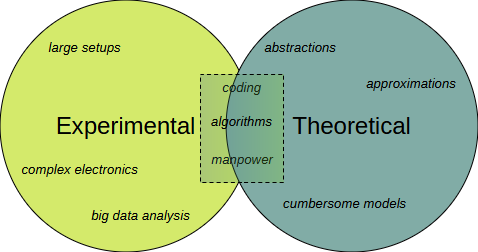
\includegraphics[scale=0.7]{figures/exp_vs_theory.png}
    \end{figure}
\end{frame}

\begin{frame}
	\frametitle{Fingerprints of Triaxiality}
	\begin{block}{Evidence \faSearch}
		\begin{itemize}
			\item Currently, there are \textbf{only two} well-established phenomena uniquely attributed to triaxial deformation.
			\begin{enumerate}
				\item Wobbling Motion WM (\emph{Bohr and Mottelson, 1950s})
				\item Chiral Motion $\chi$M (\emph{Frauendorf, 1997})
			\end{enumerate}
			\item These two can be measured/detected experimentally.
		\end{itemize}
	\end{block}
	\begin{alertblock}{Experimental observations \faSearch}
		First experimental evidence for \textbf{nuclear wobbling motion} in 2001.
	\end{alertblock}
	\begin{exampleblock}{\textbf{Goal} \faClipboard}
		\textbf{Describe the elusive character of Wobbling Motion in the context of nuclear triaxiality.}
	\end{exampleblock}
\end{frame}


\begin{frame}
	\frametitle{\faSearch Probing triaxiality in nuclei}
    Triaxial nuclei can be observed/obtained in several experiments:
    \begin{itemize}
        \item Nuclear fission: $A\ \rightarrow\ B\ +\ C$
        \item Nuclear fusion: $X\ +\ Y\ \rightarrow\ Z$
        \item \textbf{Fusion-evaporation reactions}: {\color{red}Long-lived} + {\color{red}enhanced deformation}
        \vspace{-0.3cm}
        \begin{align}
            {\color{blue}Beam(N_1,E)}\ +\ {\color{magenta}Target(N_2)}\longrightarrow N_3^*\rightarrow\dots\rightarrow {\color{purple}triaxial(N_4)} \nonumber
        \end{align}
    \end{itemize}
    \begin{figure}
        \centering
        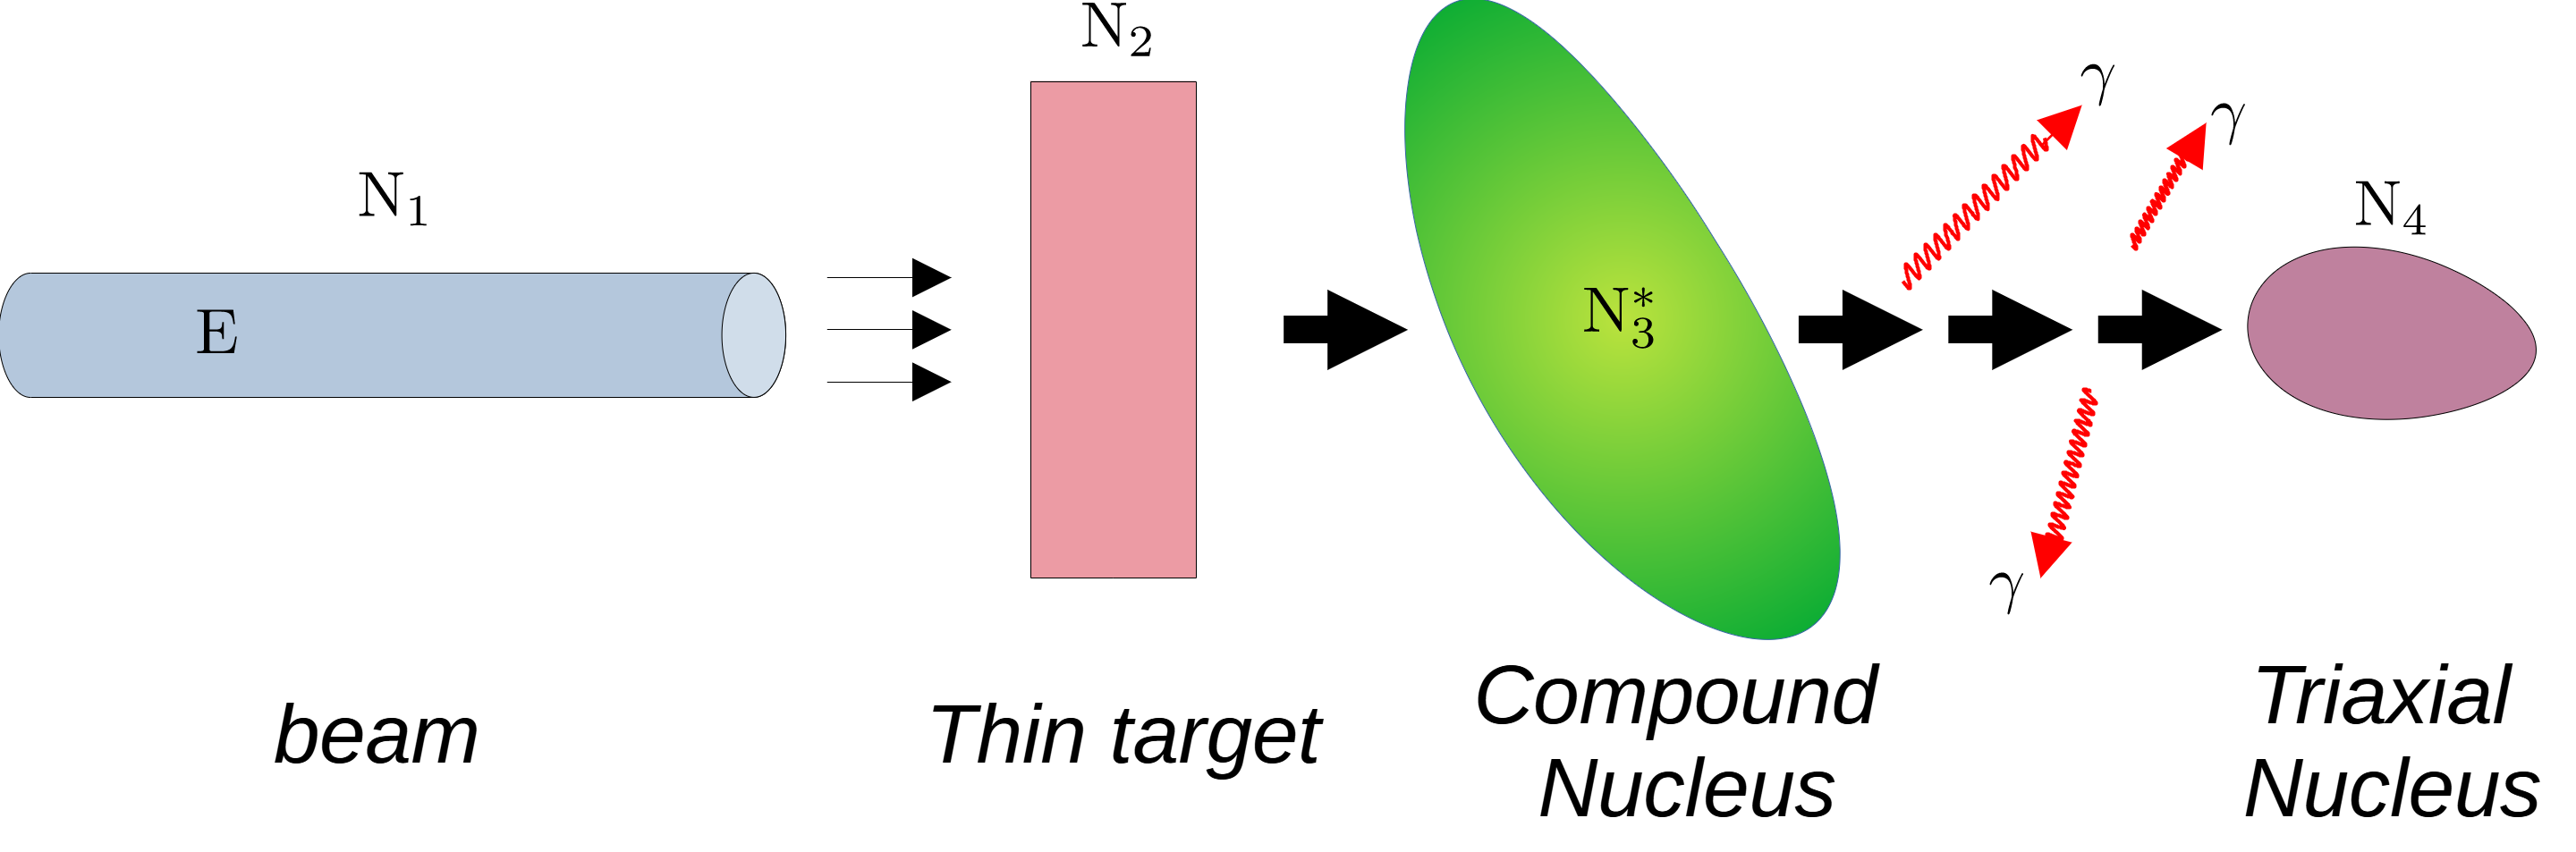
\includegraphics[scale=0.6]{figures/fusion-evaporation.png}
        % \includesvg{figures/fusion-evaporation.svg}
    \end{figure}
\end{frame}

\begin{frame}
	\frametitle{\faSearch Nuclear facilities}
	\begin{columns}
		\column{0.4\textwidth}
		\begin{figure}
		\centering
		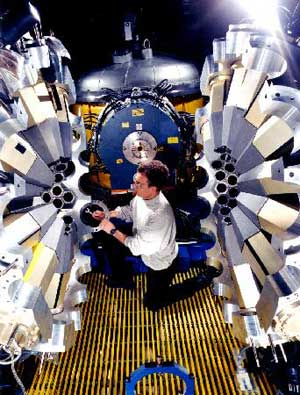
\includegraphics[width=0.86\textwidth]{figures/gsfig.jpg}
		\caption{Gammasphere detector, ANL-ATLAS USA. \textit{Source: aps.org}}
	\end{figure}
	\column{0.6\textwidth}
	\begin{figure}
		\centering
		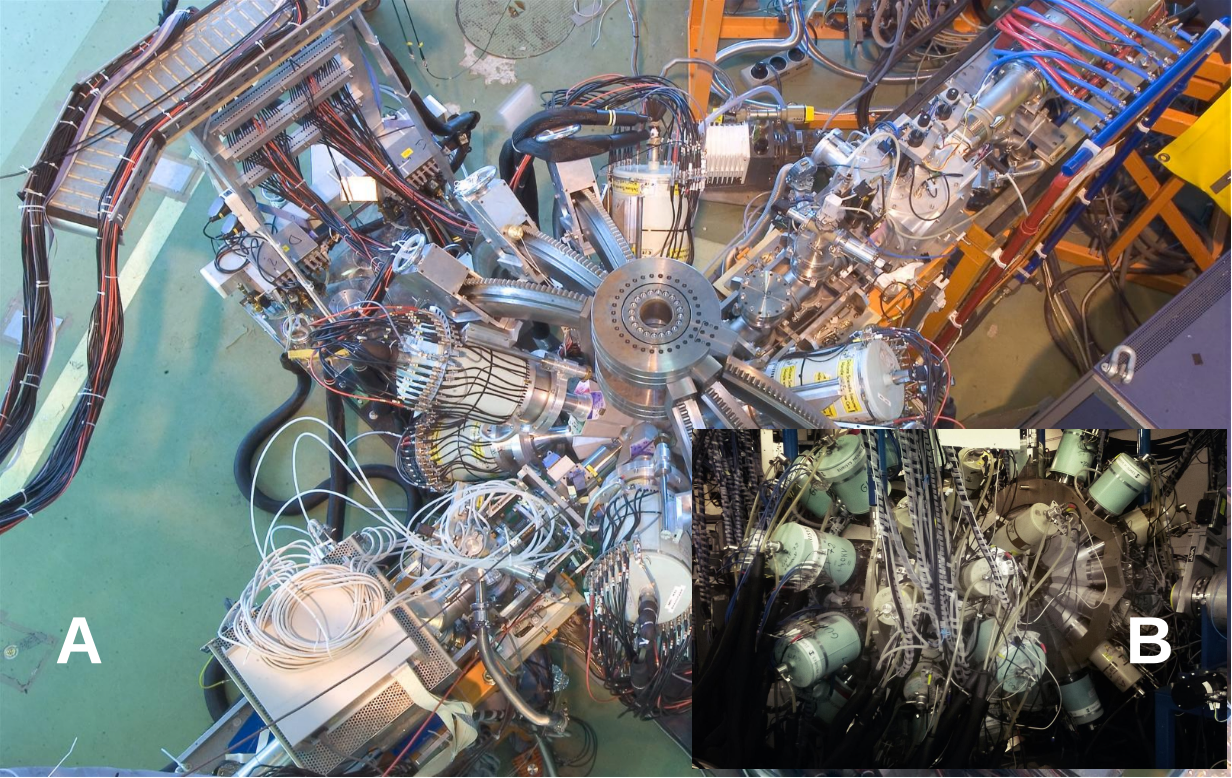
\includegraphics[width=0.98\textwidth]{figures/isolde_cern_2.png}
		\caption{a) IDS detector, CERN. \textit{Source: isolde.web.cern.ch} b) JUROGAM II, Finland. \textit{Source: twitter.com}}
		\end{figure}
	\end{columns}
\end{frame}




\section{Introduction}

% \begin{frame}
%     \transduration<0-5>{0}
%     \multiinclude[<+->][format=png, graphics={width=\textwidth}]{figures/wobbler-gif/wobbler}
%     % \animategraphics[loop,controls,width=\linewidth]{10}{figures/wobbler-gif/wobbler-}{0}{5}
% \end{frame}

\subsection{Nuclear Shapes}


\begin{frame}
	\frametitle{Nuclear Shapes (in the context of WM)}
	\begin{exampleblock}{Nuclear Radius}
		The \textbf{shape} of the nucleus is most generally described in terms of the \emph{nuclear radius}:
		\begin{align}
			R(\theta,\varphi;t)=R_0\left(1+\sum_{\lambda=0}^{^\infty}\sum_{\mu=-\lambda}^\lambda\alpha_{\lambda\mu}(t)Y_\lambda^\mu(\theta,\varphi)\right)
		\end{align}
	\end{exampleblock}
	% \begin{itemize}
	% 	\item The $\alpha_{\lambda\mu}$ are collective coordinates $\Longrightarrow$ \emph{vibrations of the nucleus}.
	% 	\item $Y_\lambda^\mu$ are the spherical harmonics.
	% \end{itemize}
	\begin{block}{Quadrupole deformations}

		\begin{itemize}
			\item {\color{red}For us:} Most relevant modes are the \textbf{quadrupole vibrations} $\lambda=2$ $\Longrightarrow$ \emph{Play a crucial role in the rotational spectra of nuclei:}
		\end{itemize}
		% \begin{align}
		% 	R(\theta,\varphi)=R_0\left(1+\sum_{\mu=-2}^2\alpha_{2\mu}Y_2^\mu(\theta,\varphi)\right)\ ,
		% \end{align}
	\end{block}
\end{frame}


\begin{frame}
	\frametitle{Axial shapes}
    \faInfo\ Most of the nuclei are either \textbf{spherical} or \textbf{axially symmetric} in their ground-state (Budaca, 2018).
	\begin{block}{Collective coordinates}
		\begin{itemize}
            \item Coordinates $\alpha_{2\mu}$ can be reduced to only two \emph{deformation parameters}: $\beta_2$ (\emph{eccentricity}) and $\gamma$ (triaxiality).
		\end{itemize}
	\end{block}
	\begin{figure}
		\centering
		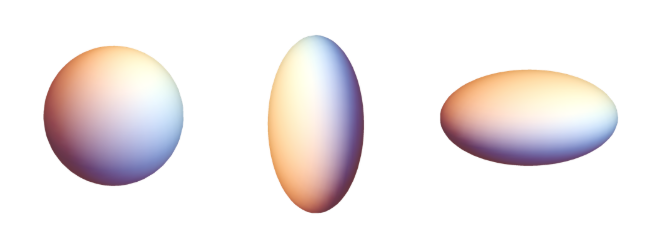
\includegraphics[scale=0.38]{figures/nuclear_shapes.png}
		\caption{\textbf{spherical:} $\beta_2=0$\ \textbf{prolate:} $\beta_2>0$\ \textbf{oblate:} $\beta_2<0$}
	\end{figure}
\end{frame}

\begin{frame}
	\frametitle{Non-axial (triaxial) shapes}
	\vspace{-0.2cm}
	\begin{alertblock}{Non-axial shapes}
		\begin{itemize}
			\item The triaxiality parameter $\gamma$ (\textit{Bohr, 1969}): departure from axial symmetry.
		\end{itemize}
	\end{alertblock}
	\vspace{-0.2cm}
	\begin{figure}
		\centering
		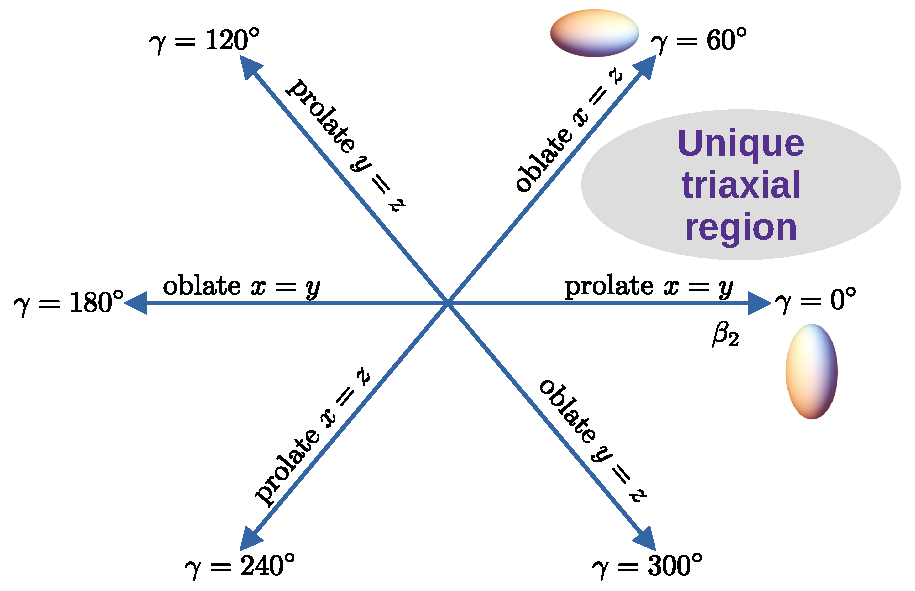
\includegraphics[scale=0.42]{figures/nice_diagram.pdf}
		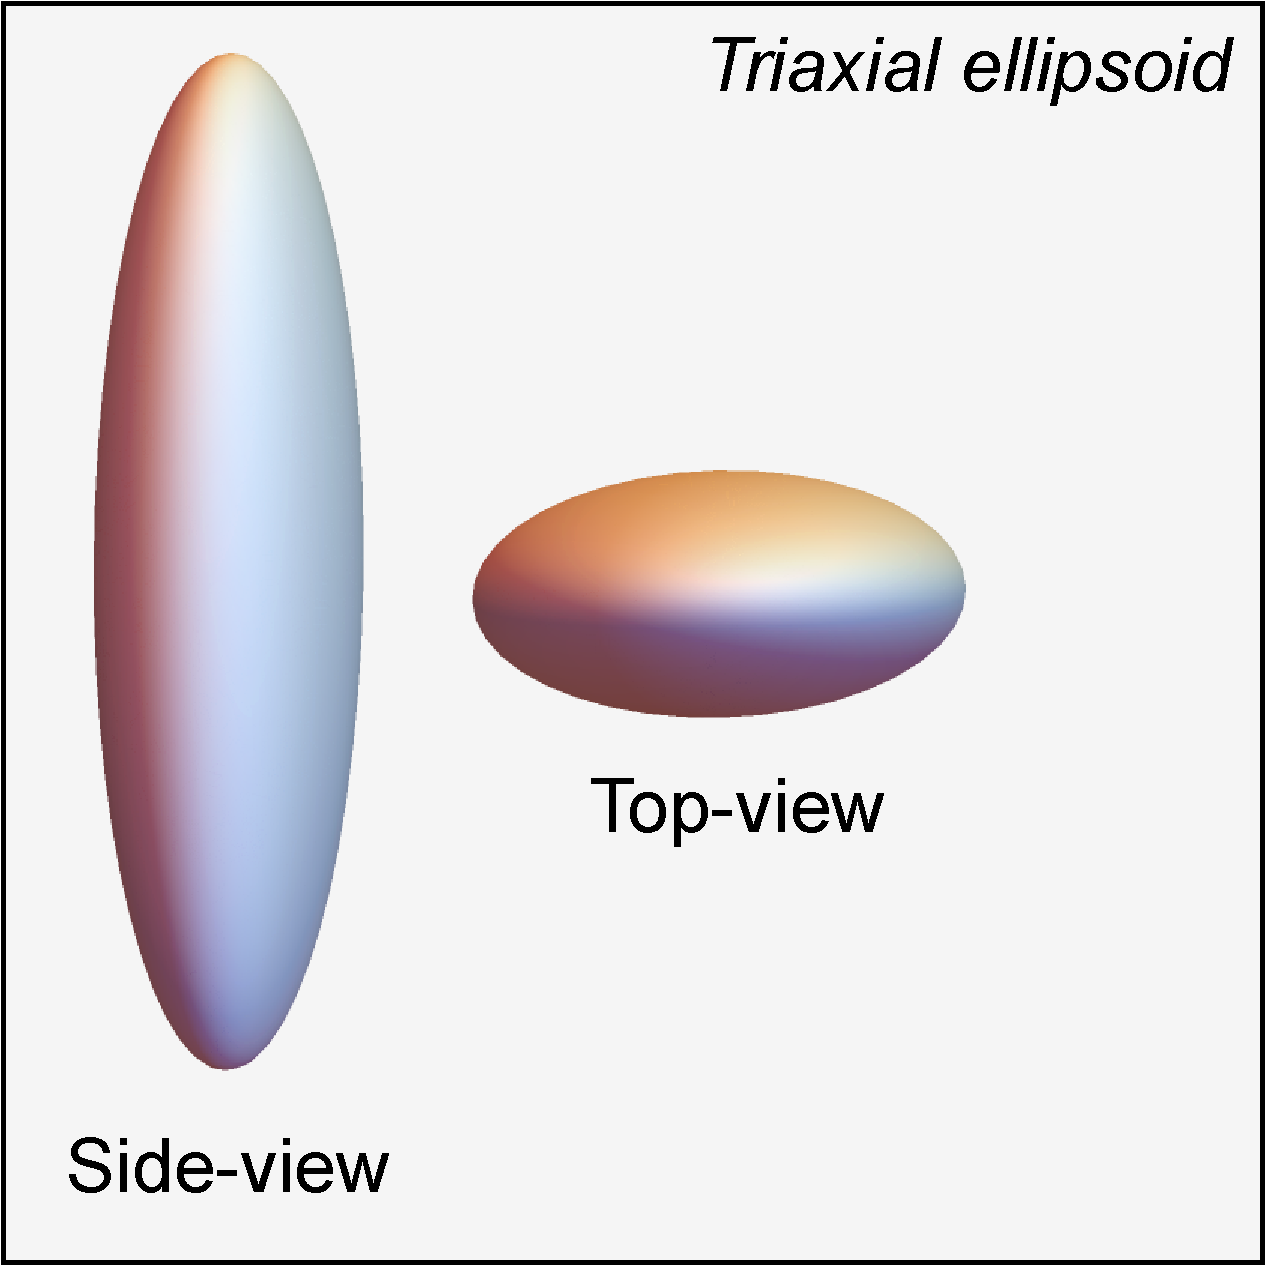
\includegraphics[scale=0.19]{figures/triaxial-shape.pdf}
		\vspace{-0.41cm}
	\end{figure}
\end{frame}


\begin{frame}[plain] % The optional argument 'plain' hides the headline and footline
	\begin{center}
		\bigskip\bigskip % Vertical whitespace
		{\Huge Thank you for your attention \faHeart}
	\end{center}
\end{frame}

\end{document}
